\chapter{Enter Numerical Methods}
\index{introduction}
\newthought{Tapping into Computational Power}


% ==============================================================================================
% INTRODUCTION BLOCK - 15 minutes

\section{The Why}\index{motivation} \index{computation} \index{Moore's Law}
\marginnote{\newthought{Further Reading}}
\newthought{Numerical Methods} \cite{arensmathematik} \cite{dahmennumerik} \cite{deisenrothmathematics} \cite{deuflhardnumerische} are essential for solving mathematical problems that cannot be addressed analytically. 
Numerical methods are a subfield of mathematics in which we calculate our solutions not analytically exactly, but approximately.


\marginnote{\newthought{Approximation} comes from Latin \textit{approximare}, meaning "to come near to".}

\newthought{And we have good reason} to do so.
\begin{itemize}
    \item Many problems cannot be solved analytically, or are too complex to be practical.
    \item We can tap into computational power to get approximate solutions efficiently.
\end{itemize} 

\marginnote{\newthought{Moore's Law \cite{moorecramming}} states that computing power doubles approximately every two years. 
As of today consumer GPUs have thousands of cores and can perform trillions of floating point operations per second.
}

% NTH: Hand-sketch a moores law diagram here.



\newthought{In machine learning and artificial intelligence,} numerical methods are crucial for training models, optimizing parameters, 
and simulating complex systems where analytical solutions are infeasible. 
They enable efficient handling of large datasets and complex algorithms, ensuring that models can learn effectively 
from data while managing computational resources. Especially in deep learning, where models involve millions of parameters and require extensive computations,
numerical methods facilitate the optimization processes that underpin model training, making them indispensable for advancing models.

\marginnote{\newthought{GPT-2: 1.5B release} \\ \url{https://openai.com/index/gpt-2-1-5b-release/}}


\newpage
\subsection{Hands On Experience}\index{analytical} \index{linear systems} \index{complexity}
Later in this course, you will learn the theoretical foundations of the numerical methods that power modern AI and ML development. 
For now let's get a feeling why these technologies lean so heavily on numerical methods.

\newthought{The limits of scaling analytical solutions} become apparent when dealing with large-scale problems.
Let's consider a simple example: Solving a system of two linear equations analytically with substitution.
\marginnote{\newthought{Analytics} includes methods like substitution, elimination, matrix inversion, etc. you would learn in linear algebra.}

\begin{equation}
    \begin{bmatrix}2 & 1 \\ 5 & 1\end{bmatrix} \begin{bmatrix}w_1 \\ w_2\end{bmatrix} = \begin{bmatrix}11 \\ 13\end{bmatrix}
\end{equation}
\label{eq:linearequation}


\begin{align*}
    \text{From the first equation:} \\
    2w_1 + w_2 &= 11 \\
    w_2 &= 11 - 2w_1 \\
    \text{Substitute into the second equation:} \\
    5w_1 + 1(11 - 2w_1) &= 13 \\
    5w_1 + 11 - 2w_1 &= 13 \\
    3w_1 + 11 &= 13 \\
    3w_1 &= 2 \\
    w_1 &= \frac{2}{3} \\
    \text{Then:} \\
    w_2 &= 11 - 2\left(\frac{2}{3}\right) \\
    &= 11 - \frac{4}{3} \\
    &= \frac{33 - 4}{3} \\
    &= \frac{29}{3} \\
    \text{Verify 1st equation:} \\
    2\left(\frac{2}{3}\right) + \left(\frac{29}{3}\right) &= \frac{4}{3} + \frac{29}{3} = \frac{33}{3} = 11 \\
    \text{Verify 2nd equation:} \\
    5\left(\frac{2}{3}\right) + 1\left(\frac{29}{3}\right) &= \frac{10}{3} + \frac{29}{3} = \frac{39}{3} = 13
\end{align*}


\marginnote{\newthought{Computational complexity} increases with the size of the system. 
Now take a shot and solve this larger system of three equations with three unknowns:

\begin{equation}
    \begin{bmatrix}
    2 & 1 & 3 \\
    1 & 4 & 2 \\
    3 & 2 & 5
    \end{bmatrix}
    \begin{bmatrix}
    w_1 \\
    w_2 \\
    w_3
    \end{bmatrix}
    =
    \begin{bmatrix}
    14 \\
    20 \\
    32
    \end{bmatrix}
\end{equation}
}

\newthought{However}, solvable for 2 equations, as the size of the system increases (e.g., thousands of equations with thousands of unknowns),
analytical solutions become impractical due to computational complexity and time constraints.

\newthought{The limits of analytical solutions} then are also a general issue in nonlinear equations:

\begin{equation}
            \sigma(x) = \frac{1}{1 + e^{-x}}. 
\end{equation}
\vspace{1em}

\marginnote{\newthought{Sigma} $\sigma(x)$ is the sigmoid activation function commonly used in neural networks, and a transcendental function. 
A closed-form solution for $\sigma(x) = 0$ does not exist. $\sigma(x)$ approaches 0 asymptotically as $x$ approaches negative infinity, but never actually reaches 0 for any finite value of $x$.}

%NTH: Plot of Sigmoid function here.

Transcendental functions cannot be expressed as finite combinations of algebraic operations (addition, subtraction, multiplication, division, and roots) and thus lack closed-form solutions.
The exponential term makes it impossible to isolate $x$ using elementary functions like polynomials, rationals, or trigonometric functions.



\vspace{2.5em}
\newthought{The Learning Objectives} of this chapter aim at providing you with the abilities to:
\begin{itemize}
    \item Explain when we deploy numerical methods and the problems that come with solving problems analytically.
    \item Discretization by transforming continuous mathematical problems into discrete, computer-solvable approximations.
    \item Apply basic numerical techniques to simple problems by hand, and crunch larger problems on a computer.
\end{itemize}





% ==============================================================================================
% MAIN THEORY BLOCK - 15 minutes

\newpage
\section{Discretization and Approximation}\index{discretization} \index{approximation} \index{stepsize} \index{interval}


\begin{figure}[h]
    \centering
    % Requires: \usepackage{pgfplots}
    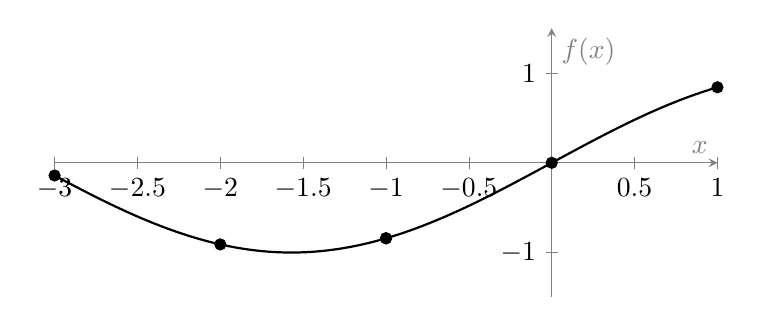
\begin{tikzpicture}
        \begin{axis}[
              width=10cm,
              height=5cm,
              axis x line=middle,
              axis y line=middle,
              xlabel={$x$},
              ylabel={$f(x)$},
              domain=-3:1,
              samples=100,
              ymin=-1.5, ymax=1.5,
              xmin=-3, xmax=1,
              legend style={at={(0.5,-0.2)},anchor=north},
              tick style={gray},
              label style={gray},
              axis line style={gray},
        ]
        % Continuous curve
        \addplot[black, thick, smooth] {sin(deg(x))};
        % Discretized points
        \addplot[black, only marks, mark=*] coordinates {
            (-3, -0.1411)
            (-2, -0.9093)
            (-1, -0.8415)
            (0, 0)
            (-1, -0.8415)
            (1, 0.8415)
        };
        \end{axis}
    \end{tikzpicture}
    \caption{Continuous curve $f(x) = \sin(x)$ and its discretized version (black dots) on $[-3,1]$ with step size $h=1$.}
    \label{fig:discretizationoverlay}
\end{figure}

\newthought{Discretization} involves breaking
continuous domains, such as time, space, or other functions,
into finite steps or grids, and evaluating these
functions at discrete points with finite precision:

\marginnote{\newthought{Remember}, the brackets $"["$ and $"]"$, are called a closed interval and mean that they include the values $a$ and $b$ in the definition set.}

\begin{align*}
    \text{Continuous function:}\quad &f(x),\quad x \in [a, b],\\
    \text{Discretized function:}\quad &f(x_i),\quad x_i = a + i h,\quad i = 0, 1, \ldots, N,
\end{align*}

where 

\begin{equation}
    h = \frac{b-a}{N},
\end{equation}

\vspace{1.5em}
is the step size, with $N$ being the number of steps on the interval.


\newthought{To analytically find} the Minimum of $\sin(x)$ on $[-3,1]$ we seek
 $\min_{x \in [-3,1]} \sin(x)$. The minimum of $\sin(x)$ occurs where its derivative vanishes and the second derivative is positive.

\begin{figure}[h]
    \centering
    % Requires: \usepackage{pgfplots}
    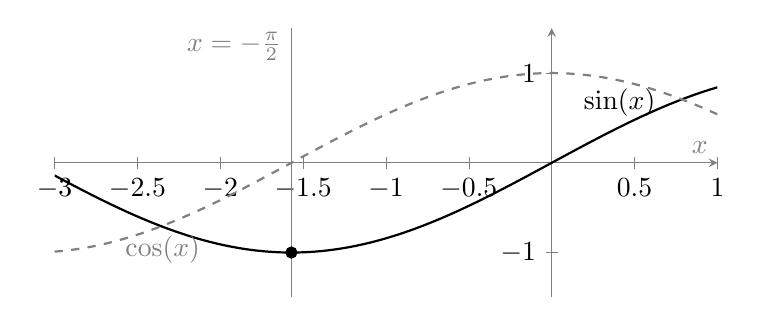
\begin{tikzpicture}
        \begin{axis}[
              width=10cm,
              height=5cm,
              axis x line=middle,
              axis y line=middle,
              xlabel={$x$},
              domain=-3:1,
              samples=100,
              ymin=-1.5, ymax=1.5,
              xmin=-3, xmax=1,
              legend style={at={(0.5,-0.2)},anchor=north},
              tick style={gray},
              label style={gray},
              axis line style={gray},
        ]
        % Continuous curve
        \addplot[black, thick, smooth] {sin(deg(x))} 
            node[pos=0.85, above] {$\sin(x)$};
        % Derivative curve (dashed)
        \addplot[gray, thick, dashed, smooth] {cos(deg(x))} 
            node[pos=0.15, below] {$\cos(x)$};
        % Discretized points (analytical minimum)
            \addplot[black, only marks, mark=*] coordinates {
                (-1.5708, -1)
            };
               % Thin solid gray line at x = -pi/2
                \addplot[gray] coordinates {
                    (-1.5708, -1.5)
                    (-1.5708, 1.5)
                };
                % Annotation for the vertical line at x = -pi/2
                \node[gray, left] at (axis cs:-1.5708,1.3) {$x = -\frac{\pi}{2}$};
        \end{axis}
    \end{tikzpicture}
    \caption{Continuous curve $f(x)=\sin(x)$ (black), its derivative $f'(x)=\cos(x)$ (gray, dashed), 
    and the analytical minimum (black dot) on $[-3,1]$. The dashed gray line marks the critical point where $\cos(x)=0$ 
    and the minimum of $\sin(x)$.}
    \label{fig:analyticallyfindingmin}
\end{figure}
 

\begin{align*}
    &f(x) = \sin(x) \\
    &f'(x) = \cos(x) = 0 \implies x^* = \frac{\pi}{2} + k\pi,\ k \in \mathbb{Z}
\end{align*}

\marginnote{\newthought{Trigonometric Rules} give us this general solution for $\cos(x) = 0$. If you forget you can always derive it from the unit circle.}
% NTH: Unit circle sketch here.

Within $[-3,1]$, the critical points are:
\begin{align*}
    x_1 = -\frac{\pi}{2} \approx -1.5708 \\
    x_2 = \frac{\pi}{2} \approx 1.5708\ (>1,\ \text{not in interval})
\end{align*}

\vspace{1.5em}
The minimum (or maximum) of a function on a closed interval $[a, b]$ can occur at a critical point 
(where the derivative is zero or undefined) inside the interval, 
or at the endpoints $a$ or $b$ themselves, even if the derivative at the endpoints is not zero. 
This is why, when searching for extrema on a closed interval, you must check both the critical points and the endpoints.\\


\begin{align*}
    \text{Check endpoints and $x_1$: } \\
    \sin(-3) &\approx -0.1411 \\
    \sin(-\frac{\pi}{2}) &= -1 \\
    \sin(1) &\approx 0.8415
\end{align*}
Thus, the minimum is $-1$ at $x = -\frac{\pi}{2} \approx -1.5708$.

\marginnote{\newthought{Brute Force} means we try out all possible options and select the best one. Here with a grid search.}


\vspace{1em}
\newthought{On To the Numerical Solution}, here we use a brute force grid search. When doing a grid search, we evaluate the function 
at discrete points over the interval and select the point with the minimum value. Discretizes $[-3,1]$ with step size $h=1$.

\begin{figure}[h]
    \centering
    % Requires: \usepackage{pgfplots}
    \begin{tikzpicture}
        \begin{axis}[
              width=10cm,
              height=5cm,
              axis x line=middle,
              axis y line=middle,
              xlabel={$x$},
              ylabel={$f(x)$},
              domain=-3:1,
              samples=100,
              ymin=-1.5, ymax=1.5,
              xmin=-3, xmax=1,
              legend style={at={(0.5,-0.2)},anchor=north},
              tick style={gray},
              label style={gray},
              axis line style={gray},
        ]
        % Discretized points
        \addplot[black, only marks, mark=*] coordinates {
            (-3, -0.1411)
            (-2, -0.9093)
            (-1, -0.8415)
            (0, 0)
            (1, 0.8415)
        };
        \end{axis}
    \end{tikzpicture}
    \caption{Continuous curve $f(x) = \sin(x)$ and its discretized version (black dots) on $[-3,1]$ with step size $h=1$.}
    \label{fig:discretization}
\end{figure}


\marginnote{\newthought{The minimum} among these is $\sin(-2) \approx -0.9093$ at $x=-2$. 
It is easy to see that the choice of step size $h$ affects the accuracy of the approximation. 
A smaller step size would yield a closer approximation to the true minimum. 
Further the interval selection matters, in a sense that it .\newthought{Approximation Error} is the difference between the analytical and numerical solutions. Here: $|-1 - (-0.9093)| = 0.0907$.}


\begin{align*}
    x_0 &= -3, & \sin(-3) &\approx -0.1411 \\
    x_1 &= -2, & \sin(-2) &\approx -0.9093 \\
    x_2 &= -1, & \sin(-1) &\approx -0.8415 \\
    x_3 &= 0, & \sin(0) &= 0 \\
    x_4 &= 1, & \sin(1) &\approx 0.8415
\end{align*}
Thus, the minimum among these is $\sin(-2) \approx -0.9093$ at $x=-2$.











% ==============================================================================================
% STUDENT ACTIVATION BLOCK - 15 minutes

\newpage
\section{Examples \& Excercises}\index{examples} \index{exercises} \index{grid search} \index{error}

\marginnote{\newthought{Excercises} are for practice and reinforcing concepts. Try to solve them on your own first, 
try things, play with it, discuss, this is not a time trial. And there is no shame in not ending up at the right answer, 
in the same sense, that uncovering great questions 
and tossing them around is usually pretty fruitful on the long run.}

\newthought{Remember,} our example from above?

\marginnote{\newthought{Linear regression} see how $xw+b$ forms a linear model, which can also be thought of as the most basic form of a single unit neural network $\theta$.}

\begin{equation}
    \begin{bmatrix}2 & 1 \\ 5 & 1\end{bmatrix} \begin{bmatrix}w \\ b\end{bmatrix} = \begin{bmatrix}11 \\ 13\end{bmatrix}
\end{equation}
\newthought{This we} can also solve via brute force discretization and approximation.
We discretize the variables $w$ and $b$ over a grid of possible values, solve according to these values and select 
the solution that minimizes the error.
\newthought{Let's perform a grid search} for $w$ and $b$ with step size $2.5$ over the range $w, b \in \{0, 2.5, 5, 7.5, 10\}$. For each combination, we compute the error:

\newthought{Error} is defined as the sum of absolute differences between the left and right sides of the equations:
\begin{equation}
    \begin{aligned}
        \text{error}_1 &= \left|2w + b - 11\right|, \\
        \text{error}_2 &= \left|5w + b - 13\right|.
    \end{aligned}
\end{equation}




We evaluate all combinations and select the $(w, b)$ pair with the smallest accumulated error.


\newthought{There is value in} doing this by hand, as it helps to understand the mechanics of numerical methods. Also it gives an intuition 
on the computeational cost of brute-force methods, and later on we will find more efficient approaches. This was only $100$ operations, and it does not fail to bring the message home that
this is something you will want to hand over and automate on a computer. Which on the other hand does not even struggle with this size of a problem.


\newthought{Enter the machine.} A lot of numerical methods are designed to be implemented on computers. 
In this lecture course, we will often switch between hand calculations for small examples and computer implementations for larger problems.

\marginnote{\newthought{Code is hosted as notebooks} and is to be followed up here \url{https://enlitenment.schutera.com/landing}.}
\newthought{You get} a jupyter notebook pre-hosted at your fingertips. With it you get a python template for this excercise. Use the self-reflection questions below to guide your while exploring and experimenting with the implementation. 



\begin{table*}[ht]
\centering
\begin{tabular}{p{0.08\textwidth}p{0.08\textwidth}p{0.22\textwidth}p{0.22\textwidth}p{0.18\textwidth}}
\toprule
\textbf{$w$} & \textbf{$b$} & $2w + b$ ($error_1$) & $5w + b$ ($error_2$) & \textbf{Error} \\
\midrule
0   & 0   & 0 \hspace{0.5em} (11)   & 0 \hspace{0.5em} (13)   & 24 \\
0   & 2.5 & 2.5 \hspace{0.5em} (8.5) & 2.5 \hspace{0.5em} (10.5) & 19 \\
0   & 5   & 5 \hspace{0.5em} (6)     & 5 \hspace{0.5em} (8)     & 14 \\
0   & 7.5 & 7.5 \hspace{0.5em} (3.5) & 7.5 \hspace{0.5em} (5.5) & 9 \\
0   & 10  & 10 \hspace{0.5em} (1)    & 10 \hspace{0.5em} (3)    & 4* \\
2.5 & 0   & 5 \hspace{0.5em} (6)     & 12.5 \hspace{0.5em} (0.5) & 6.5 \\
2.5 & 2.5 & 7.5 \hspace{0.5em} (3.5) & 15 \hspace{0.5em} (2)     & 5.5 \\
2.5 & 5   & 10 \hspace{0.5em} (1)    & 17.5 \hspace{0.5em} (4.5) & 5.5 \\
2.5 & 7.5 & 12.5 \hspace{0.5em} (1.5) & 20 \hspace{0.5em} (7)     & 8.5 \\
2.5 & 10  & 15 \hspace{0.5em} (4)    & 22.5 \hspace{0.5em} (9.5) & 13.5 \\
5   & 0   & 10 \hspace{0.5em} (1)    & 25 \hspace{0.5em} (12)    & 13 \\
5   & 2.5 & 12.5 \hspace{0.5em} (1.5) & 27.5 \hspace{0.5em} (14.5) & 16 \\
5   & 5   & 15 \hspace{0.5em} (4)    & 30 \hspace{0.5em} (17)    & 21 \\
5   & 7.5 & 17.5 \hspace{0.5em} (6.5) & 32.5 \hspace{0.5em} (19.5) & 26 \\
5   & 10  & 20 \hspace{0.5em} (9)    & 35 \hspace{0.5em} (22)    & 31 \\
7.5 & 0   & 15 \hspace{0.5em} (4)    & 37.5 \hspace{0.5em} (24.5) & 28.5 \\
7.5 & 2.5 & 17.5 \hspace{0.5em} (6.5) & 40 \hspace{0.5em} (27)     & 33.5 \\
7.5 & 5   & 20 \hspace{0.5em} (9)    & 42.5 \hspace{0.5em} (29.5) & 38.5 \\
7.5 & 7.5 & 22.5 \hspace{0.5em} (11.5) & 45 \hspace{0.5em} (32)    & 43.5 \\
7.5 & 10  & 25 \hspace{0.5em} (14)   & 47.5 \hspace{0.5em} (34.5) & 48.5 \\
10  & 0   & 20 \hspace{0.5em} (9)    & 50 \hspace{0.5em} (37)     & 46 \\
10  & 2.5 & 22.5 \hspace{0.5em} (11.5) & 52.5 \hspace{0.5em} (39.5) & 51 \\
10  & 5   & 25 \hspace{0.5em} (14)   & 55 \hspace{0.5em} (42)     & 56 \\
10  & 7.5 & 27.5 \hspace{0.5em} (16.5) & 57.5 \hspace{0.5em} (44.5) & 61 \\
10  & 10  & 30 \hspace{0.5em} (19)   & 60 \hspace{0.5em} (47)     & 66 \\
\bottomrule
\end{tabular}
\vspace{2em}
\caption{Grid search for $w, b$ in $\{0, 2.5, 5, 7.5, 10\}$: values of $2w + b$ and $5w + b$ with errors to 11 and 13 in parentheses. The last column shows the accumulated error (sum of absolute errors). 
The minimum error occurs at $w = 0$, $b = 10$ with an error of 4 (marked with *).}
\label{tab:gridsearch}
\end{table*}



\section{Self-Reflection and Recap}\index{reflection} \index{recap} \index{error}

%<Discussion about the findings and the learned concepts>
\newthought{Self-Reflection} Questions which can guide your thoughts during the excercises and afterwards:
\begin{itemize}
    \item Why is the choice of step size $h$ important when discretizing a continuous function, and how does it affect the accuracy and the compute time of the numerical solution?
    \item How does the selection of the interval $[a, b]$ influence the results of discretization and the location of extrema found numerically?
    \item What are the main differences between a continuous function and its discretized version, and what are the implications for solving mathematical problems numerically?
\end{itemize}

%<Recap of Key Concepts>
\newthought{Recap} of Key Concepts:
\begin{itemize}
    \item Numerical Methods are essential for solving complex mathematical problems that lack analytical solutions.
    \item Discretization transforms continuous problems into discrete approximations suitable for computational methods.
    \item We can do numerical computations by hand for small problems to understand the mechanics, but computers are essential for larger problems.
\end{itemize}


\newthought{Errors everywhere.} Mathematical models are simplifications of reality, 
and numerical methods introduce additional errors through approximation.

\marginnote{\newthought{Teaser.} Can you think of a simple way to improve the accuracy to compute ratio of our grid search example from above?}

\begin{equation}
    f(x) \approx f(x_i),\quad x_i = a + i h
\end{equation}

Numerical computation introduces a few types of errors, which we will need to understand in order to 
be able to fully harness this new methodology.





%%%%%%%%%%%%%%%%%%%%%%%%%%%%%%%%%%%%%%%%%%%%%%%%%%%%%%%%%%%%%%%%%%%%%%%%%%%%%%







































